\documentclass[12pt,a4paper]{article}
\usepackage[UTF8]{ctex}
\usepackage{amsmath,amssymb}
\usepackage{listings}
\usepackage{xcolor}
\usepackage{hyperref}
\usepackage{geometry}
\usepackage{graphicx}
\geometry{margin=2.5cm}

\lstdefinestyle{python}{
  language=Python,
  basicstyle=\ttfamily\small,
  keywordstyle=\color{blue}\bfseries,
  commentstyle=\color{gray},
  stringstyle=\color{red},
  showstringspaces=false,
  breaklines=true,
  frame=single,
  backgroundcolor=\color{gray!10}
}

\title{HHL Algorithm / HHL 算法}
\author{QuoNic}
\date{}

\begin{document}
\maketitle

\begin{center}
\textbf{Algorithms / 算法} | 难度：高级 | 预计时间：25 分钟
\end{center}

\tableofcontents
\newpage

\section{为什么需要？}

HHL 算法用于求解线性方程组 $Ax=b$，提供指数加速。

\subsection{经典局限}
\begin{itemize}
  \item 经典算法（如高斯消元）需要 $O(N^3)$ 时间
  \item 对于大规模稀疏矩阵，经典方法效率低
\end{itemize}

\subsection{量子优势}
\begin{itemize}
  \item HHL 算法需要 $O(\text{poly}(\log N))$ 时间
  \item 对于稀疏矩阵，提供指数加速
  \item 是量子机器学习的基础
\end{itemize}

\subsection{实际应用}
\begin{itemize}
  \item 线性方程组求解
  \item 量子机器学习
  \item 量子模拟
\end{itemize}

\section{快速上手}

\begin{lstlisting}[style=python]
from quonic.algorithms import hhl

# Solve Ax = b
A = [[1, 0], [0, 2]]
b = [1, 1]
result = hhl(A, b)
print(f"Solution: {result.x}")
\end{lstlisting}

\textbf{预期输出}：
\begin{verbatim}
Solution: [1.0, 0.5]
\end{verbatim}

\section{原理详解}

\subsection{电路图}

\begin{center}
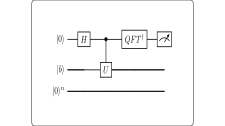
\includegraphics[width=0.7\textwidth]{../../images/hhl_circuit.svg}
\end{center}

\subsection{数学推导}

HHL 算法求解 $Ax=b$：
\begin{equation}
|x\rangle = A^{-1}|b\rangle
\end{equation}

\textbf{算法步骤}：
\begin{enumerate}
  \item 用 QPE 估计 $A$ 的本征值
  \item 用受控旋转将本征值取倒数
  \item 用逆 QPE 恢复量子态
  \item 测量得到解 $|x\rangle$
\end{enumerate}

\textbf{复杂度}：
\begin{equation}
O(\text{poly}(\log N) \cdot \kappa^2 / \epsilon)
\end{equation}

其中 $\kappa$ 是条件数，$\epsilon$ 是精度。

\subsection{几何解释}

HHL 算法在量子态空间中操作，通过 QPE 将矩阵对角化，然后取倒数得到解。

\section{代码详解}

\begin{lstlisting}[style=python]
from quonic.algorithms import hhl

# hhl(A, b)
# A: coefficient matrix
# b: right-hand side vector
result = hhl(A, b)

# result.x: solution vector
# result.condition_number: condition number of A
print(f"Solution: {result.x}")
\end{lstlisting}

\section{进阶用法}

\subsection{场景 1：不同矩阵}

\begin{lstlisting}[style=python]
# Different matrices
A1 = [[1, 2], [3, 4]]
b1 = [1, 0]
result1 = hhl(A1, b1)

A2 = [[1, 0, 0], [0, 2, 0], [0, 0, 3]]
b2 = [1, 1, 1]
result2 = hhl(A2, b2)
\end{lstlisting}

\section{适用场景}

\subsection{线性方程组求解}

HHL 算法可以高效求解大规模稀疏线性方程组。

\subsection{量子机器学习}

HHL 算法是量子机器学习的基础组件。

\section{常见问题}

\subsection{HHL 算法的加速比是多少？}

指数加速：$O(\text{poly}(\log N))$ vs $O(N^3)$。

\subsection{HHL 算法的局限性是什么？}

HHL 算法需要矩阵是稀疏的，且条件数不能太大。

\section{学习路径}

\subsection{前置知识}
\begin{itemize}
  \item 量子相位估计（QPE）
  \item 量子傅里叶变换（QFT）
  \item 线性代数
\end{itemize}

\subsection{继续学习}
\begin{itemize}
  \item 量子机器学习
  \item 量子模拟
  \item 量子优化
\end{itemize}

\section{完整示例代码}

\subsection{示例 1：基本 HHL}

\begin{lstlisting}[style=python]
from quonic.algorithms import hhl

A = [[1, 0], [0, 2]]
b = [1, 1]
result = hhl(A, b)
print(f"Solution: {result.x}")
\end{lstlisting}

\end{document}
